% --- Use 'standalone' class to crop the output to the figure ---
\documentclass[tikz, border=5pt]{standalone}

% --- Load TikZ Libraries ---
\usepackage{tikz}
\usetikzlibrary{arrows.meta} % For nicer arrow tips
\usepackage{amsfonts} % FIX: Load package for \mathbb

\begin{document}

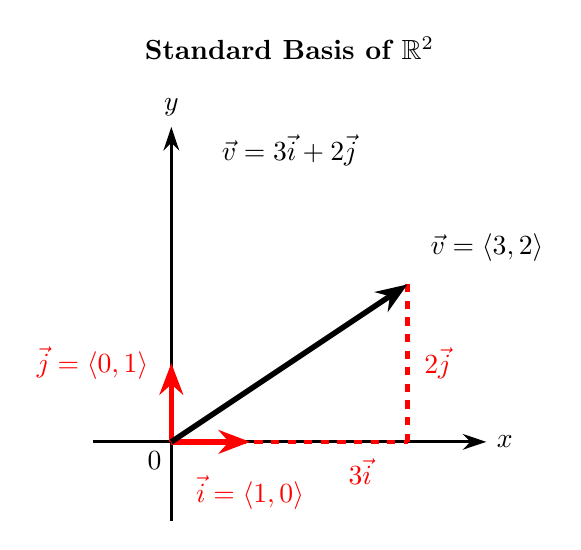
\begin{tikzpicture}[
    font=\sffamily,
    % Style for the main vectors
    vec/.style={
        line width=2pt,
        -{Stealth[length=4mm, width=3mm]}
    },
    % Style for the components/construction lines
    comp/.style={
        line width=1.5pt,
        dashed
    }
]

% --- Draw Axes ---
% We draw them slightly extended
\draw[-{Stealth[length=3mm, width=2mm]}, line width=1pt] (-1,0) -- (4,0) node[right] {$x$};
\draw[-{Stealth[length=3mm, width=2mm]}, line width=1pt] (0,-1) -- (0,4) node[above] {$y$};
\node[below left] at (0,0) {$0$};

% --- 1. Draw Basis Vector i ---
% MODIFIED: Moved label further down
\draw[vec, red] (0,0) -- (1,0) node[below=8pt] {$\vec{i} = \langle1, 0\rangle$};

% --- 2. Draw Basis Vector j ---
\draw[vec, red] (0,0) -- (0,1) node[left=4pt] {$\vec{j} = \langle0, 1\rangle$};

% --- 3. Show an example vector v = (3, 2) ---
\coordinate (v) at (3, 2); % Define the point
\coordinate (vx) at (3, 0); % x-component
\coordinate (vy) at (0, 2); % y-component

% --- 4. Show the components a*i and b*j ---
% Draw 3*i component
% MODIFIED: Changed 'midway' to 'pos=0.8' to shift label right
\draw[comp, red] (0,0) -- (vx) node[pos=0.8, below=2pt] {$3\vec{i}$};
% Draw 2*j component
\draw[comp, red] (vx) -- (v) node[midway, right=2pt] {$2\vec{j}$};

% --- 5. Draw the final vector v ---
\draw[vec, black] (0,0) -- (v) node[above right=4pt] {$\vec{v} = \langle3, 2\rangle$};

% --- Add a title/label for the whole figure ---
% MODIFIED: Moved title and equation up
\node[font=\bfseries] at (1.5, 5.0) {Standard Basis of $\mathbb{R}^2$};
\node at (1.5, 3.7) {$\vec{v} = 3\vec{i} + 2\vec{j}$};


\end{tikzpicture}

\end{document}